\subsection{\textbf{Sistema de controle de versões}}

Durante o processo de desenvolvimento de \textit{software}, a etapa de codificação gera várias linhas de códigos. Além disso, modificações e melhorias no \textit{software} ocorrem constantemente no decorrer do tempo, seja a pedido do usuário ou alguma possível atualização.  As equipes de desenvolvimento são compostas por vários tipos de desenvolvedores, cada um com sua personalidade e experiência. Sendo assim, os desenvolvimentos de \textit{softwares} são feitos por etapas, onde cada desenvolvedor é responsável por entregar o que foi designado a ele. 

Devido a isso, para organizar essas etapas de desenvolvimento, utiliza-se ferramentas que gerencia e controla diferentes versões de \textit{software}.  Segundo \citeonline{OReilly},  uma ferramenta que realiza o gerenciamento e o controle de versões de \textit{software} ou outro conteúdo “é referida genericamente como um VCS - \textit{Version Control System} (Sistema de controle de versão ), um SCM - \textit{Source Code Manager} (Gerenciador de código-fonte) ou um RCS - \textit{Revision Control System} (Sistema de controle de revisão)”. Essas ferramentas controlam quais linhas de códigos foram alteradas, qual contribuidor do projeto fez a alteração, o horário da alteração, dentre outros. Além do mais, essas ferramentas possibilitam aos desenvolvedores uma opção de voltar o código para versões anteriores, caso algum \textit{bug} (problema) na versão atual do sistema cause algum transtorno.

\citeonline{OReilly} enfatizam que nenhuma pessoa criativa e cautelosa inicia um projeto sem um método de \textit{backup}. Sendo assim, outra funcionalidade muito importante que as ferramentas de rastreamento e gerenciamento de código proporcionam para os desenvolvedores são os repositórios de \textit{backup}, que mantêm hospedado de forma segura todas os arquivos relacionados ao sistema desenvolvido.

\subsubsection{\textit{Git}}

Basicamente, o \textit{Git} é um sistema distribuído e de código aberto que controla versões de arquivos desenvolvidos, no qual possui diversos comandos que auxilia os desenvolvedores a realizar projetos de grade e pequeno porte com velocidade e eficiência.  Com esses comandos, o \textit{Git} disponibiliza um amplo conjunto de ferramentas para realizar a manipulação dos arquivos no seu repositório local ou \textit{Web}, garantindo a integridade dos dados \cite{GIT2010}.

A \autoref{fig_git} demostra um exemplo da utilização de comandos \textit{git} para controlar um repositório local ou \textit{web}.

\begin{figure}[h]
	\caption{\label{fig_git}Exemplo de comandos \textit{Git}.}
	\begin{center}
		\resizebox{1\linewidth}{!}{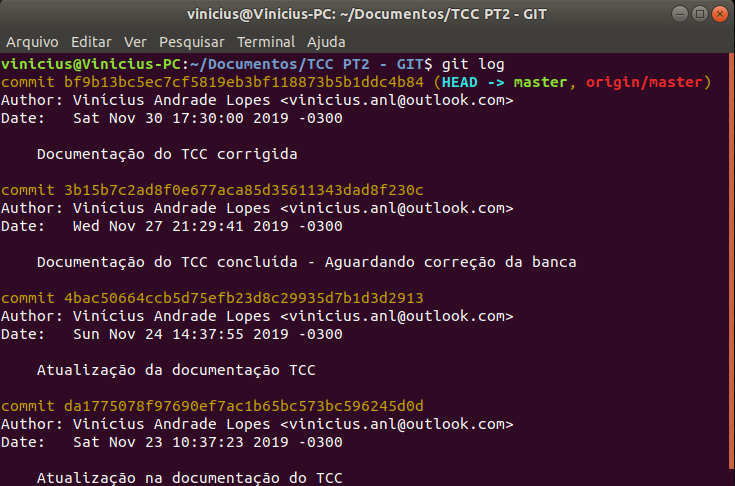
\includegraphics{4-Conteudo-Bibliografico/4-Ferramentas-de-Desenvolvimento-do-Projeto/git.png}}
	\end{center}
	\centering \legend{Fonte: Elaborada pelos autores.}
\end{figure}

Segundo \citeonline{CHACON2014}, o maior diferencial do sistema de controle de versões \textit{Git} é o seu modelo de ramificação (\textit{branch}), que possibilita ao usuário a criação de uma cópia do sistema principal. Com essa cópia, o desenvolvedor pode realizar implementações de melhorias/correções em trechos de códigos sem modificar a aplicação principal. Depois da implementação e dos testes, o desenvolvedor pode substituir a \textit{branch} principal (\textit{master}) pela \textit{branch} com implementações. Os únicos arquivos que serão substituídos serão os arquivos editados.
\subsubsection{\textit{GitHub}}


Já o \textit{GitHub} é uma plataforma de hospedagem de códigos que utiliza o \textit{Git} como controle de versão. O \textit{GitHub} possui uma grande interação com repositórios \textit{Git}, concentrando uma grande comunidade de desenvolvedores que colaboram para milhões de projetos \cite{CHACON2014}.

Ainda segundo \citeonline{CHACON2014}, o \textit{GitHub} hospeda a maior porcentagem de repositórios \textit{Git}. Isso ocorre porque a plataforma também disponibiliza recursos de gerenciamento de código, como por exemplo o rastreamento de problemas, revisão de código, edição \textit{online} do código, dentre outros.